% This file was created by tikzplotlib v0.8.7.
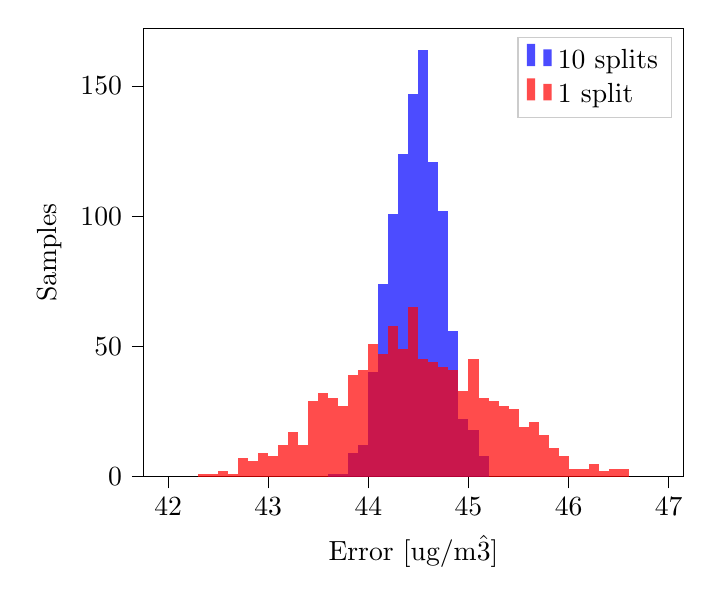
\begin{tikzpicture}

\begin{axis}[
legend cell align={left},
legend style={fill opacity=0.8, draw opacity=1, text opacity=1, draw=white!80.0!black},
tick align=outside,
tick pos=left,
x grid style={white!69.01960784313725!black},
xlabel={Error [ug/m\^3]},
xmin=41.755, xmax=47.1450000000001,
xtick style={color=black},
y grid style={white!69.01960784313725!black},
ylabel={Samples},
ymin=0, ymax=172.2,
ytick style={color=black}
]
\draw[fill=blue,draw opacity=0,fill opacity=0.7] (axis cs:42,0) rectangle (axis cs:42.1,0);
\addlegendimage{ybar,ybar legend,fill=blue,draw opacity=0,fill opacity=0.7};
\addlegendentry{10 splits}

\draw[fill=blue,draw opacity=0,fill opacity=0.7] (axis cs:42.1,0) rectangle (axis cs:42.2,0);
\draw[fill=blue,draw opacity=0,fill opacity=0.7] (axis cs:42.2,0) rectangle (axis cs:42.3,0);
\draw[fill=blue,draw opacity=0,fill opacity=0.7] (axis cs:42.3,0) rectangle (axis cs:42.4,0);
\draw[fill=blue,draw opacity=0,fill opacity=0.7] (axis cs:42.4,0) rectangle (axis cs:42.5,0);
\draw[fill=blue,draw opacity=0,fill opacity=0.7] (axis cs:42.5,0) rectangle (axis cs:42.6,0);
\draw[fill=blue,draw opacity=0,fill opacity=0.7] (axis cs:42.6,0) rectangle (axis cs:42.7,0);
\draw[fill=blue,draw opacity=0,fill opacity=0.7] (axis cs:42.7,0) rectangle (axis cs:42.8,0);
\draw[fill=blue,draw opacity=0,fill opacity=0.7] (axis cs:42.8,0) rectangle (axis cs:42.9,0);
\draw[fill=blue,draw opacity=0,fill opacity=0.7] (axis cs:42.9,0) rectangle (axis cs:43,0);
\draw[fill=blue,draw opacity=0,fill opacity=0.7] (axis cs:43,0) rectangle (axis cs:43.1,0);
\draw[fill=blue,draw opacity=0,fill opacity=0.7] (axis cs:43.1,0) rectangle (axis cs:43.2,0);
\draw[fill=blue,draw opacity=0,fill opacity=0.7] (axis cs:43.2,0) rectangle (axis cs:43.3,0);
\draw[fill=blue,draw opacity=0,fill opacity=0.7] (axis cs:43.3,0) rectangle (axis cs:43.4,0);
\draw[fill=blue,draw opacity=0,fill opacity=0.7] (axis cs:43.4,0) rectangle (axis cs:43.5,0);
\draw[fill=blue,draw opacity=0,fill opacity=0.7] (axis cs:43.5,0) rectangle (axis cs:43.6,0);
\draw[fill=blue,draw opacity=0,fill opacity=0.7] (axis cs:43.6,0) rectangle (axis cs:43.7,1);
\draw[fill=blue,draw opacity=0,fill opacity=0.7] (axis cs:43.7,0) rectangle (axis cs:43.8,1);
\draw[fill=blue,draw opacity=0,fill opacity=0.7] (axis cs:43.8,0) rectangle (axis cs:43.9,9);
\draw[fill=blue,draw opacity=0,fill opacity=0.7] (axis cs:43.9,0) rectangle (axis cs:44,12);
\draw[fill=blue,draw opacity=0,fill opacity=0.7] (axis cs:44,0) rectangle (axis cs:44.1,40);
\draw[fill=blue,draw opacity=0,fill opacity=0.7] (axis cs:44.1,0) rectangle (axis cs:44.2,74);
\draw[fill=blue,draw opacity=0,fill opacity=0.7] (axis cs:44.2,0) rectangle (axis cs:44.3,101);
\draw[fill=blue,draw opacity=0,fill opacity=0.7] (axis cs:44.3,0) rectangle (axis cs:44.4,124);
\draw[fill=blue,draw opacity=0,fill opacity=0.7] (axis cs:44.4,0) rectangle (axis cs:44.5,147);
\draw[fill=blue,draw opacity=0,fill opacity=0.7] (axis cs:44.5,0) rectangle (axis cs:44.6,164);
\draw[fill=blue,draw opacity=0,fill opacity=0.7] (axis cs:44.6,0) rectangle (axis cs:44.7,121);
\draw[fill=blue,draw opacity=0,fill opacity=0.7] (axis cs:44.7,0) rectangle (axis cs:44.8,102);
\draw[fill=blue,draw opacity=0,fill opacity=0.7] (axis cs:44.8,0) rectangle (axis cs:44.9,56);
\draw[fill=blue,draw opacity=0,fill opacity=0.7] (axis cs:44.9,0) rectangle (axis cs:45,22);
\draw[fill=blue,draw opacity=0,fill opacity=0.7] (axis cs:45,0) rectangle (axis cs:45.1,18);
\draw[fill=blue,draw opacity=0,fill opacity=0.7] (axis cs:45.1000000000001,0) rectangle (axis cs:45.2000000000001,8);
\draw[fill=blue,draw opacity=0,fill opacity=0.7] (axis cs:45.2,0) rectangle (axis cs:45.3,0);
\draw[fill=blue,draw opacity=0,fill opacity=0.7] (axis cs:45.3000000000001,0) rectangle (axis cs:45.4000000000001,0);
\draw[fill=blue,draw opacity=0,fill opacity=0.7] (axis cs:45.4,0) rectangle (axis cs:45.5,0);
\draw[fill=blue,draw opacity=0,fill opacity=0.7] (axis cs:45.5000000000001,0) rectangle (axis cs:45.6000000000001,0);
\draw[fill=blue,draw opacity=0,fill opacity=0.7] (axis cs:45.6000000000001,0) rectangle (axis cs:45.7000000000001,0);
\draw[fill=blue,draw opacity=0,fill opacity=0.7] (axis cs:45.7000000000001,0) rectangle (axis cs:45.8000000000001,0);
\draw[fill=blue,draw opacity=0,fill opacity=0.7] (axis cs:45.8000000000001,0) rectangle (axis cs:45.9000000000001,0);
\draw[fill=blue,draw opacity=0,fill opacity=0.7] (axis cs:45.9000000000001,0) rectangle (axis cs:46.0000000000001,0);
\draw[fill=blue,draw opacity=0,fill opacity=0.7] (axis cs:46.0000000000001,0) rectangle (axis cs:46.1000000000001,0);
\draw[fill=blue,draw opacity=0,fill opacity=0.7] (axis cs:46.1000000000001,0) rectangle (axis cs:46.2000000000001,0);
\draw[fill=blue,draw opacity=0,fill opacity=0.7] (axis cs:46.2000000000001,0) rectangle (axis cs:46.3000000000001,0);
\draw[fill=blue,draw opacity=0,fill opacity=0.7] (axis cs:46.3000000000001,0) rectangle (axis cs:46.4000000000001,0);
\draw[fill=blue,draw opacity=0,fill opacity=0.7] (axis cs:46.4000000000001,0) rectangle (axis cs:46.5000000000001,0);
\draw[fill=blue,draw opacity=0,fill opacity=0.7] (axis cs:46.5000000000001,0) rectangle (axis cs:46.6000000000001,0);
\draw[fill=blue,draw opacity=0,fill opacity=0.7] (axis cs:46.6000000000001,0) rectangle (axis cs:46.7000000000001,0);
\draw[fill=blue,draw opacity=0,fill opacity=0.7] (axis cs:46.7000000000001,0) rectangle (axis cs:46.8000000000001,0);
\draw[fill=blue,draw opacity=0,fill opacity=0.7] (axis cs:46.8000000000001,0) rectangle (axis cs:46.9000000000001,0);
\draw[fill=red,draw opacity=0,fill opacity=0.7] (axis cs:42,0) rectangle (axis cs:42.1,0);
\addlegendimage{ybar,ybar legend,fill=red,draw opacity=0,fill opacity=0.7};
\addlegendentry{1 split}

\draw[fill=red,draw opacity=0,fill opacity=0.7] (axis cs:42.1,0) rectangle (axis cs:42.2,0);
\draw[fill=red,draw opacity=0,fill opacity=0.7] (axis cs:42.2,0) rectangle (axis cs:42.3,0);
\draw[fill=red,draw opacity=0,fill opacity=0.7] (axis cs:42.3,0) rectangle (axis cs:42.4,1);
\draw[fill=red,draw opacity=0,fill opacity=0.7] (axis cs:42.4,0) rectangle (axis cs:42.5,1);
\draw[fill=red,draw opacity=0,fill opacity=0.7] (axis cs:42.5,0) rectangle (axis cs:42.6,2);
\draw[fill=red,draw opacity=0,fill opacity=0.7] (axis cs:42.6,0) rectangle (axis cs:42.7,1);
\draw[fill=red,draw opacity=0,fill opacity=0.7] (axis cs:42.7,0) rectangle (axis cs:42.8,7);
\draw[fill=red,draw opacity=0,fill opacity=0.7] (axis cs:42.8,0) rectangle (axis cs:42.9,6);
\draw[fill=red,draw opacity=0,fill opacity=0.7] (axis cs:42.9,0) rectangle (axis cs:43,9);
\draw[fill=red,draw opacity=0,fill opacity=0.7] (axis cs:43,0) rectangle (axis cs:43.1,8);
\draw[fill=red,draw opacity=0,fill opacity=0.7] (axis cs:43.1,0) rectangle (axis cs:43.2,12);
\draw[fill=red,draw opacity=0,fill opacity=0.7] (axis cs:43.2,0) rectangle (axis cs:43.3,17);
\draw[fill=red,draw opacity=0,fill opacity=0.7] (axis cs:43.3,0) rectangle (axis cs:43.4,12);
\draw[fill=red,draw opacity=0,fill opacity=0.7] (axis cs:43.4,0) rectangle (axis cs:43.5,29);
\draw[fill=red,draw opacity=0,fill opacity=0.7] (axis cs:43.5,0) rectangle (axis cs:43.6,32);
\draw[fill=red,draw opacity=0,fill opacity=0.7] (axis cs:43.6,0) rectangle (axis cs:43.7,30);
\draw[fill=red,draw opacity=0,fill opacity=0.7] (axis cs:43.7,0) rectangle (axis cs:43.8,27);
\draw[fill=red,draw opacity=0,fill opacity=0.7] (axis cs:43.8,0) rectangle (axis cs:43.9,39);
\draw[fill=red,draw opacity=0,fill opacity=0.7] (axis cs:43.9,0) rectangle (axis cs:44,41);
\draw[fill=red,draw opacity=0,fill opacity=0.7] (axis cs:44,0) rectangle (axis cs:44.1,51);
\draw[fill=red,draw opacity=0,fill opacity=0.7] (axis cs:44.1,0) rectangle (axis cs:44.2,47);
\draw[fill=red,draw opacity=0,fill opacity=0.7] (axis cs:44.2,0) rectangle (axis cs:44.3,58);
\draw[fill=red,draw opacity=0,fill opacity=0.7] (axis cs:44.3,0) rectangle (axis cs:44.4,49);
\draw[fill=red,draw opacity=0,fill opacity=0.7] (axis cs:44.4,0) rectangle (axis cs:44.5,65);
\draw[fill=red,draw opacity=0,fill opacity=0.7] (axis cs:44.5,0) rectangle (axis cs:44.6,45);
\draw[fill=red,draw opacity=0,fill opacity=0.7] (axis cs:44.6,0) rectangle (axis cs:44.7,44);
\draw[fill=red,draw opacity=0,fill opacity=0.7] (axis cs:44.7,0) rectangle (axis cs:44.8,42);
\draw[fill=red,draw opacity=0,fill opacity=0.7] (axis cs:44.8,0) rectangle (axis cs:44.9,41);
\draw[fill=red,draw opacity=0,fill opacity=0.7] (axis cs:44.9,0) rectangle (axis cs:45,33);
\draw[fill=red,draw opacity=0,fill opacity=0.7] (axis cs:45,0) rectangle (axis cs:45.1,45);
\draw[fill=red,draw opacity=0,fill opacity=0.7] (axis cs:45.1000000000001,0) rectangle (axis cs:45.2000000000001,30);
\draw[fill=red,draw opacity=0,fill opacity=0.7] (axis cs:45.2,0) rectangle (axis cs:45.3,29);
\draw[fill=red,draw opacity=0,fill opacity=0.7] (axis cs:45.3000000000001,0) rectangle (axis cs:45.4000000000001,27);
\draw[fill=red,draw opacity=0,fill opacity=0.7] (axis cs:45.4,0) rectangle (axis cs:45.5,26);
\draw[fill=red,draw opacity=0,fill opacity=0.7] (axis cs:45.5000000000001,0) rectangle (axis cs:45.6000000000001,19);
\draw[fill=red,draw opacity=0,fill opacity=0.7] (axis cs:45.6000000000001,0) rectangle (axis cs:45.7000000000001,21);
\draw[fill=red,draw opacity=0,fill opacity=0.7] (axis cs:45.7000000000001,0) rectangle (axis cs:45.8000000000001,16);
\draw[fill=red,draw opacity=0,fill opacity=0.7] (axis cs:45.8000000000001,0) rectangle (axis cs:45.9000000000001,11);
\draw[fill=red,draw opacity=0,fill opacity=0.7] (axis cs:45.9000000000001,0) rectangle (axis cs:46.0000000000001,8);
\draw[fill=red,draw opacity=0,fill opacity=0.7] (axis cs:46.0000000000001,0) rectangle (axis cs:46.1000000000001,3);
\draw[fill=red,draw opacity=0,fill opacity=0.7] (axis cs:46.1000000000001,0) rectangle (axis cs:46.2000000000001,3);
\draw[fill=red,draw opacity=0,fill opacity=0.7] (axis cs:46.2000000000001,0) rectangle (axis cs:46.3000000000001,5);
\draw[fill=red,draw opacity=0,fill opacity=0.7] (axis cs:46.3000000000001,0) rectangle (axis cs:46.4000000000001,2);
\draw[fill=red,draw opacity=0,fill opacity=0.7] (axis cs:46.4000000000001,0) rectangle (axis cs:46.5000000000001,3);
\draw[fill=red,draw opacity=0,fill opacity=0.7] (axis cs:46.5000000000001,0) rectangle (axis cs:46.6000000000001,3);
\draw[fill=red,draw opacity=0,fill opacity=0.7] (axis cs:46.6000000000001,0) rectangle (axis cs:46.7000000000001,0);
\draw[fill=red,draw opacity=0,fill opacity=0.7] (axis cs:46.7000000000001,0) rectangle (axis cs:46.8000000000001,0);
\draw[fill=red,draw opacity=0,fill opacity=0.7] (axis cs:46.8000000000001,0) rectangle (axis cs:46.9000000000001,0);
\end{axis}

\end{tikzpicture}
